
\documentclass[12pt]{article}
\usepackage[utf8]{inputenc}
\usepackage{graphicx}
\usepackage{float}
\usepackage{geometry}
\geometry{margin=1in}
\title{Informe Visualizaciones - Tecnología}
\author{Grupo 19}
\date{Junio 2025}

\begin{document}

\maketitle

\section*{Visualización 1: Porcentaje de personas que usan internet en el mundo (Tarea 1)}

\begin{figure}[H]
    \centering
    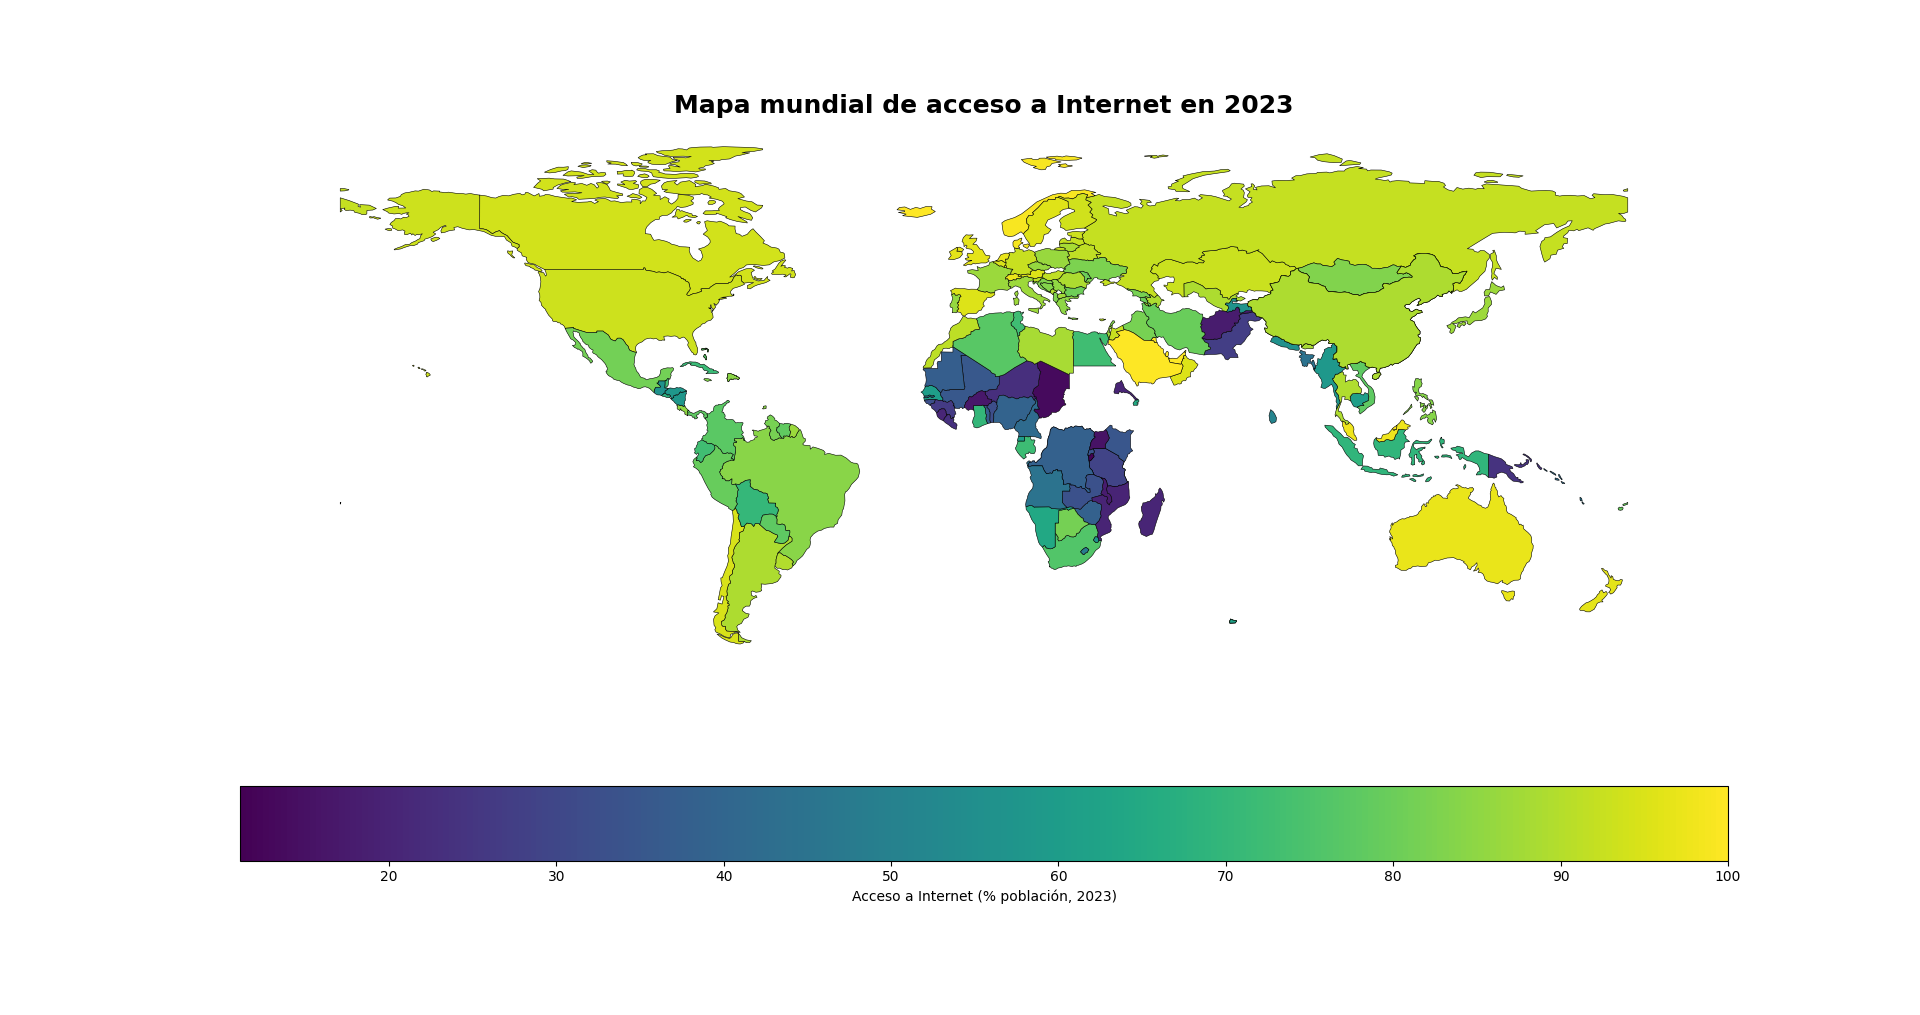
\includegraphics[width=0.8\textwidth]{images/uso_internet.png}
    \caption{Fuente: World Bank (https://data.worldbank.org/indicator/IT.NET.USER.ZS)}
\end{figure}

\begin{itemize}
  \item \textbf{Visualización:} Mapa Coroplético Mundial
  \item \textbf{Marca:} Mapa mundial de acceso a Internet en 2023
  \item \textbf{Fuente de datos:} Datos internacionales sobre porcentaje de población con acceso a Internet por país (posiblemente ITU, World Bank o Our World in Data)
  \item \textbf{Herramienta utilizada:} Python (GeoPandas, Matplotlib)
\end{itemize}

\subsubsection*{Canales Visuales}
\begin{itemize}
  \item \textbf{Color:} Escala secuencial continua desde púrpura oscuro (bajo acceso) hasta amarillo brillante (alto acceso)
  \item \textbf{Posición:} Geográfica, respetando la ubicación real de los países
  \item \textbf{Área:} Constante (los países no cambian de tamaño)
  \item \textbf{Leyenda:} Barra continua con valores entre 10\% y 100\% de acceso
\end{itemize}

\begin{figure}[H]
    \centering
    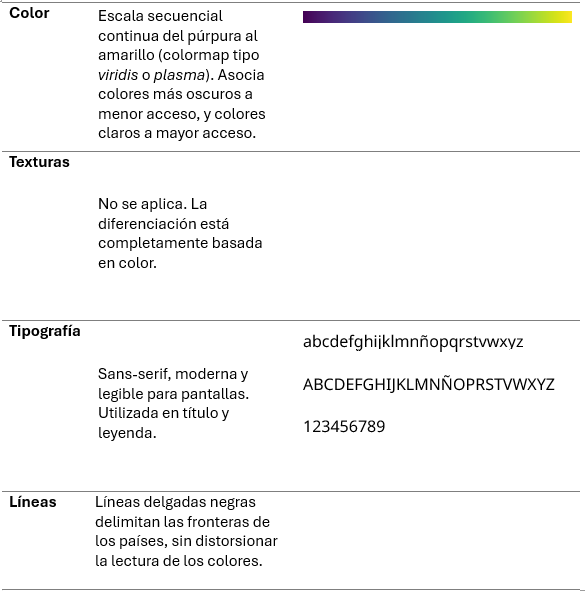
\includegraphics[width=0.8\textwidth]{images/Ficha_Calor.png}
    \caption{Ficha tecnica del mapa de calor.}
\end{figure}

\subsection*{Integrante responsable}
Felipe Campaña
\newpage

\newpage

\section*{Visualización 2: Popularidad de redes sociales globales}

\begin{figure}[H]
    \centering
    \caption{Fuente: RAWGraphs – Kaggle (Social Media Usage)}
\end{figure}

\begin{itemize}
  \item \textbf{Visualización:} Diagrama de caja (Boxplot).
  \item \textbf{Marca:} Comparación de percepción de utilidad de la IA por año de estudio.
  \item \textbf{Fuente de datos:} Encuesta a estudiantes de 1° y 2° año sobre la confianza y utilidad percibida de la inteligencia artificial.
  \item \textbf{Herramienta utilizada:} Python + librerias  \textit{seaborn}, \textit{pandas} y \textit{Matplotlib}.
\end{itemize}

\subsubsection*{Canales Visuales}
\begin{itemize}
  \item \textbf{Color:} Diferenciación visual de grupos mediante colores (verde para 1°, naranjo para 2°)
  \item \textbf{Posición:} Año de estudio en el eje X (1° y 2°), percepción de utilidad en el eje Y
  \item \textbf{Área:} No aplica directamente; los elementos del boxplot tienen tamaños estándar
  \item \textbf{Leyenda:} Mediana, cuartiles, bigotes y posibles outliers expresados gráficamente
\end{itemize}

\begin{figure}[H]
    \centering
    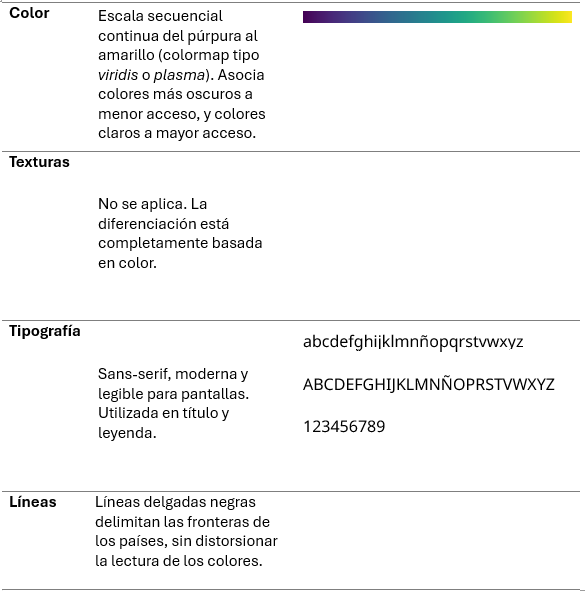
\includegraphics[width=0.8\textwidth]{images/Ficha_Calor.png}
    \caption{...}
\end{figure}

\subsection*{Integrante responsable}
Matias Elgueta
\newpage

\section*{Visualización 3: Principales usos de inteligencia artificial (Tarea 2)}

\begin{figure}[H]
    \centering
    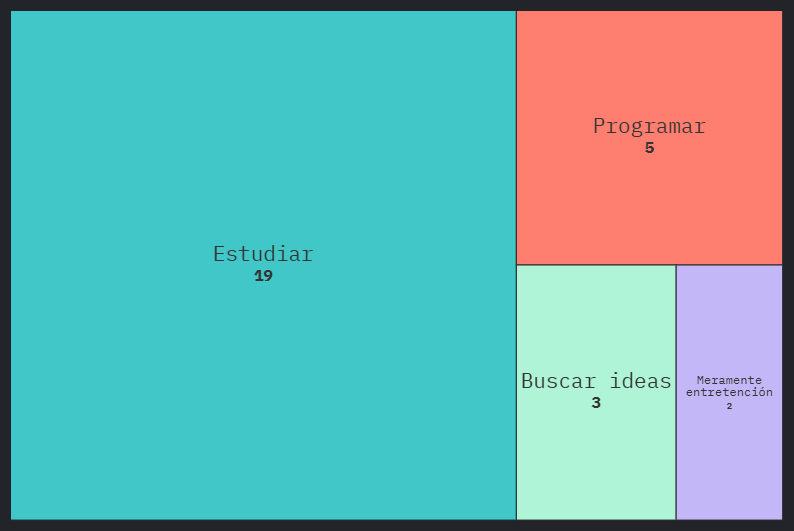
\includegraphics[width=0.8\textwidth]{images/treemap.png}
    \caption{Fuente: Elaboración propia con datos de encuesta (Google Forms)}
\end{figure}

\begin{itemize}
  \item \textbf{Visualización:} Mapa de árbol (Treemap)
  \item \textbf{Marca:} Distribución de tiempo según tipo de actividad
  \item \textbf{Fuente de datos:} Datos personales sobre uso del tiempo categorizado en actividades: Estudiar, Programar, Buscar ideas, Meramente entretención
  \item \textbf{Herramienta utilizada:} Flourish
\end{itemize}

\subsubsection*{Canales Visuales}
\begin{itemize}
  \item \textbf{Color:} Diferencia visualmente cada categoría de actividad.
  \item \textbf{Posición:} Determinada automáticamente por el algoritmo de partición.
  \item \textbf{Área:} El tamaño de cada rectángulo representa la proporción de tiempo dedicada a cada actividad.
  \item \textbf{Leyenda:} Se incluye dentro de cada bloque para indicar la categoría y su valor.
\end{itemize}

\begin{figure}[H]
    \centering
    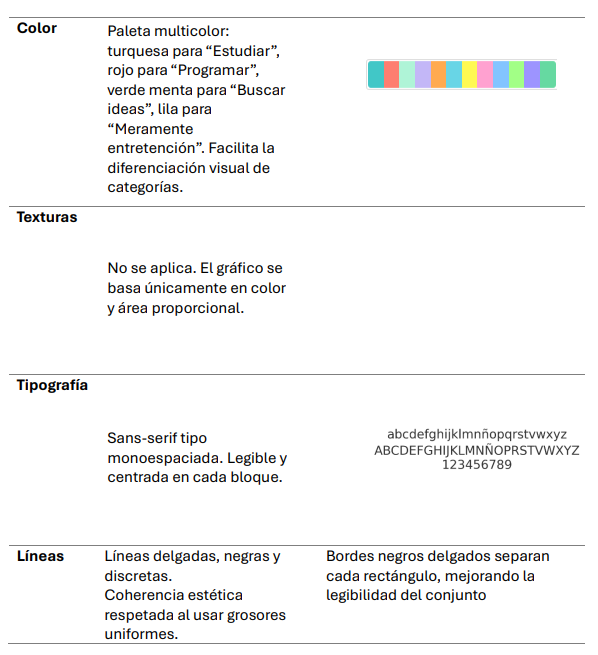
\includegraphics[width=0.8\textwidth]{images/Ficha_jg2.png}
    \caption{Ficha técnica Treemap}
\end{figure}


\subsection*{Integrante responsable}
Javier Gómez
\newpage


\section*{Visualización 4: Comparación de percepciones sobre IA en educación}

\begin{figure}[H]
    \centering
    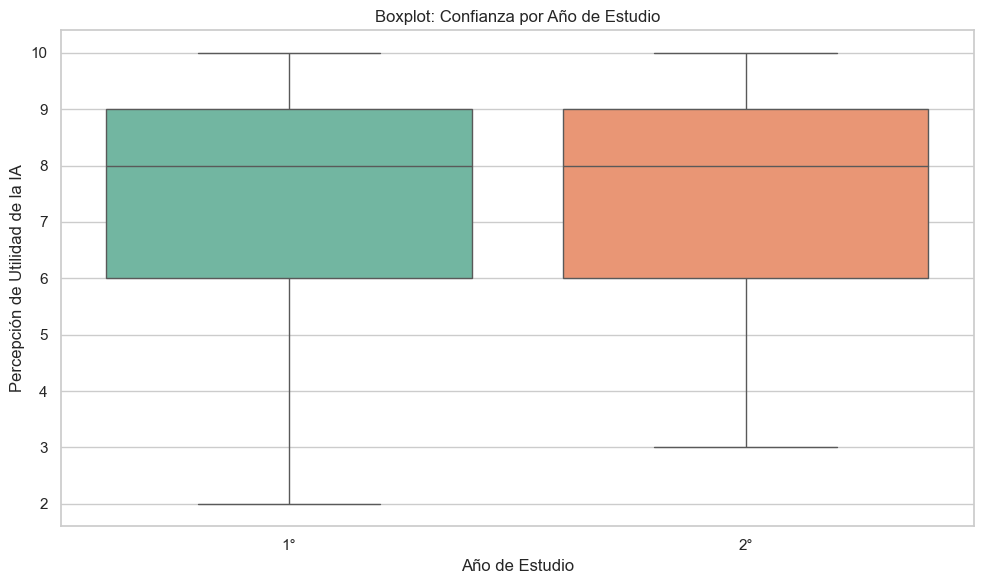
\includegraphics[width=0.8\textwidth]{images/boxplot.png}
    \caption{Fuente: Flourish – Datos de Kaggle (AI in Education Survey)}
\end{figure}

\begin{itemize}
  \item \textbf{Visualización:} Diagrama de caja (Boxplot).
  \item \textbf{Marca:} Comparación de percepción de utilidad de la IA por año de estudio.
  \item \textbf{Fuente de datos:} Encuesta a estudiantes de 1° y 2° año sobre la confianza y utilidad percibida de la inteligencia artificial.
  \item \textbf{Herramienta utilizada:} Python + librerias  \textit{seaborn}, \textit{pandas} y \textit{Matplotlib}.
\end{itemize}

\subsubsection*{Canales Visuales}
\begin{itemize}
  \item \textbf{Color:} Diferenciación visual de grupos mediante colores (verde para 1°, naranjo para 2°)
  \item \textbf{Posición:} Año de estudio en el eje X (1° y 2°), percepción de utilidad en el eje Y
  \item \textbf{Área:} No aplica directamente; los elementos del boxplot tienen tamaños estándar
  \item \textbf{Leyenda:} Mediana, cuartiles, bigotes y posibles outliers expresados gráficamente
\end{itemize}


\begin{figure}[H]
    \centering
    \includegraphics[width=0.8\textwidth]{images/ficha_jg1.png}
    \caption{Ficha técnica boxplot}
\end{figure}


\subsection*{Integrante responsable}
Javier Gómez
\newpage

\section*{Visualización 5: Flujos de ciberataques entre países}

\begin{figure}[H]
    \centering
    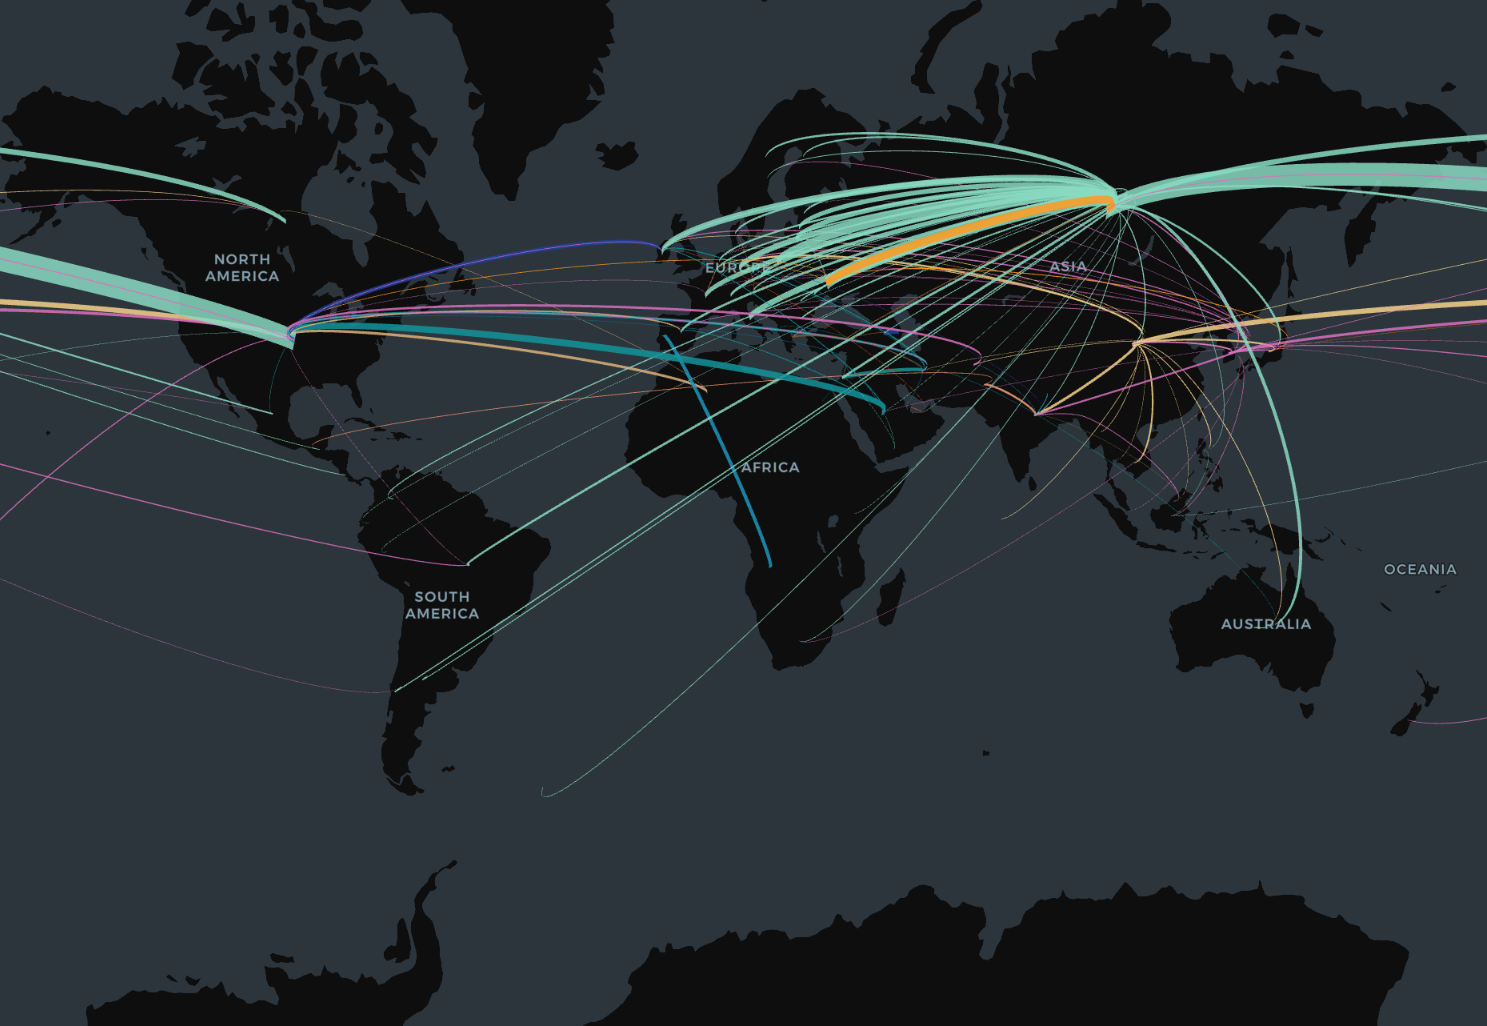
\includegraphics[width=0.8\textwidth]{images/flujo_ataque.png}
    \caption{Fuente: Kepler.gl con datos del Cyber Events Database (UMD)}
\end{figure}

\begin{itemize}
  \item \textbf{Visualización:} ...
  \item \textbf{Marca:} ...
  \item \textbf{Fuente de datos:} ...
  \item \textbf{Herramienta utilizada:} ...
\end{itemize}

\subsubsection*{Canales Visuales}
\begin{itemize}
  \item \textbf{Color:} ...
  \item \textbf{Posición:} ...
  \item \textbf{Área:} ...
  \item \textbf{Leyenda:} ...
\end{itemize}

\begin{figure}[H]
    \centering
    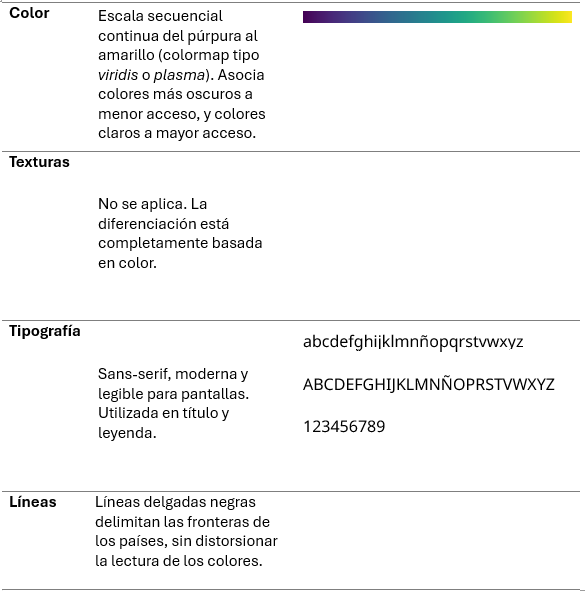
\includegraphics[width=0.8\textwidth]{images/Ficha_Calor.png}
    \caption{...}
\end{figure}

\subsection*{Integrante responsable}
Matias Elgueta
\newpage

\newpage

\section*{Visualización 6: Flujos de actores y motivos de ciberataques (Tarea 3)}

\begin{figure}[H]
    \centering
    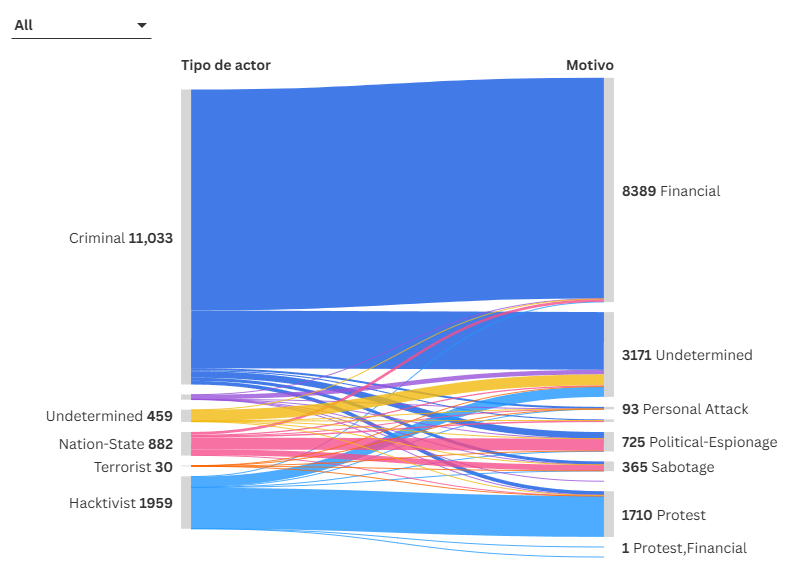
\includegraphics[width=0.8\textwidth]{images/SANKEY_FC.png}
    \caption{Fuente: Cyber Events Database (UMD)}
\end{figure}

\subsection*{Justificación de diseño visual}
\begin{itemize}
    \item \textbf{Visualización:} Gráfico de Flujo Tipo Sankey
    \item \textbf{Marca:} Visualización de Ciberataques según Tipo de Actor y Motivo.
    \item \textbf{Posición:} Eje horizontal para flujo entre categorías ("Tipo de actor" a "Motivo").
    \item \textbf{Herramienta utilizada:} Posiblemente Flourish, RAWGraphs o Tableau (basado en el estilo visual)
    \item \textbf{Color:} Diferenciación de tipos de actor.
\end{itemize}

\subsubsection*{Canales Visuales}
\begin{itemize}
  \item \textbf{Posición:} Eje horizontal para mostrar el flujo de relaciones entre categorías
  \item \textbf{Color:} Diferenciación de tipos de actor mediante colores únicos
  \item \textbf{Tamaño (grosor):} Representa el volumen de incidentes asociados a cada flujo
  \item \textbf{Conexión:} Enlace visual entre categorías (actor y motivo)
\end{itemize}

\begin{figure}[H]
    \centering
    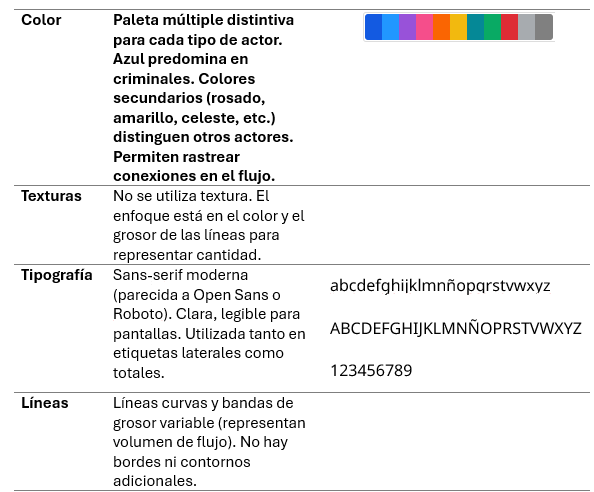
\includegraphics[width=0.8\textwidth]{images/Ficha_sankey.png}
    \caption{Ficha tecnica de la visualización Sankey}
\end{figure}

\subsection*{Integrante responsable}
Felipe Campaña
\end{document}
